%%% 卒業論文テンプレート
\documentclass[12pt,titlepage,a4j,oneside]{myjbook2}
%\documentclass[12pt,titlepage,a4j,oneside]{jbook}
\usepackage[dvipdfmx]{graphicx}
\usepackage{multirow}
\usepackage{boxedminipage}
\usepackage{cite}
\usepackage{mathtools}
\usepackage{amsmath, amssymb, amsfonts}
%\usepackage[varg]{txfonts}
%\usepackage{txfonts}
%\usepackage{showkeys}
%\pagestyle{plain}
\newlength{\esm}
\setlength{\esm}{\evensidemargin}
\setlength{\evensidemargin}{\oddsidemargin}
\setlength{\oddsidemargin}{\esm}
\setlength{\headsep}{32pt}
\begin{document}
  \begin{titlepage}
    \begin{center}
      \vspace*{1cm}
      \LARGE 2023年度 卒業論文 \\
      \vspace*{1cm}
      \Huge 人のような描き方ができる頭部の \\
      線画生成の研究 \\
      \vspace*{45mm}

      {\LARGE %\vskip2zw 
      2024年3月}
      \vspace*{10mm}
      
      {\Large
      指導教員 \\
      藤江真也 教授} \\
      \vspace*{20mm}
      \LARGE
      千葉工業大学 先進工学部 \\
      未来ロボティクス学科 \\
      \vspace*{10mm}
      {\Huge 森~田~大~雅}
    \end{center}
  \end{titlepage}

  \frontmatter
  %\baselineskip=21pt plus 4pt minus 4pt
  \baselineskip=21pt
  \tableofcontents
  \listoffigures
  \listoftables

  \setlength{\abovedisplayskip}{25pt plus0pt minus0pt}
  \setlength{\belowdisplayskip}{25pt plus0pt minus0pt}

  \mainmatter
  %--------------------------------------------------------------
  % 1章 序論
  %#! platex 000main.tex
\chapter{序論}
  \label{chap:intro}
  \section{背景}
    \label{sec:background}
	現代ではディジタルで絵を描いたり、AIが絵を生成するようになっている.	そのため、アナログで描くことに、これから意味があるのか疑問に思う人もいると思う. コンピュータを使って自分の表現したい色や絵を生成することよりも、人が数多くの鍛錬を積み、美しい絵や不思議と魅力あふれる絵を自力で描いていくことは、これからも一定の価値を持ち続けると考えられる. しかし、描く手段が増えた分、今までより狭き門になる可能性は十分にある. 
	\\\hspace{10pt}アナログの場合、たとえ見た目が同じに見えても、絵の具を使った量や混ぜた色の比率、筆のタッチの刻み方や手のぶれなどを完全に再現できることは不可能であるため、優れた絵描きの絵のオリジナリティは強く評価される.	また時間と労力は有限であるため、作品数は限られるため希少価値は高くなる. 
	\\\hspace{10pt}このように人がアナログ絵を描く価値はこれからもあり続けると考えられるが、ロボットがアナログ絵を描いた場合はどうなるだろうか. 私は、簡易的な絵であれば、ロボットに描いてもらいたい場合が存在すると考える. 例えば、ミニ黒板を用いたカフェや飲食店などの看板イラストや、地域のイベントのポスターイラストなどである. 地域のイベントでアイディアを募集するもの良いが、このようなときに簡単なイラストが描けるロボットが存在し、活用できれば時間とコストの削減が期待できる. 
  \section{本研究の目的}
    \label{sec:target}
	従来の描画ロボットの研究では描かれた絵が、どのぐらい上手く描けているかに着目している研究が多い. 例えばシンプルにエッジ抽出から人物画を描く文献\cite{1}や、エッジ抽出とハッチングから芸術的な人物画を鉛筆で描く文献\cite{2}、リモートユーザがタブレットを介してロボットに描かせる文献\cite{3}などが存在する. これらの研究では模写や芸術的な表現が可能になっているが、人のような描き方を追求したものが少ないと感じた.
	\\\hspace{10pt}また、風景や静物などは描き手によってかなり描き順に差があるが、人物画の頭部であればある程度パターンがあると考えた.  加えて、ヒトの頭部は表情が存在するため絵に様々な意味を連想させたり、静止した一場面にストーリーをもたらせたる、背景などの他の要素をより際立たせることができる. これは絵画以外の漫画にも当てはまることで、頭部を描く重要性は高い.	そこで本研究では、ある画家が描いた頭部作品の画像から描き順ができるだけ人に近い描き方をする描画ロボットを作成を行う.\\
	

	\section{本論文の構成}
    \label{sec:construction_of_this_paper}
    


  %--------------------------------------------------------------
  % 2章 関連研究
  %#! platex 000main.tex
\chapter{関連研究}
  \label{chap:related}
  
  描画ロボットの研究はあまり多くないが、マニピュレータを使った先行研究とよく用いられるエッジ検出を行うアルゴリズムに改良を加えた研究を調査した. 本研究では線画を描くためにエッジ抽出を用いている. 画像からエッジ抽出を行うとノイズがどうしてものってしまうため、ノイズをできるだけ低減できる文献がないか調査した.  
	
  \section{描画ロボットに関する研究}
    \label{sec:related_reasearch}
	文献\cite{1}では、6軸のマニピュレータロボットを用いて、シンプルにエッジ抽出から人物画を描く研究を行っているのに対し、文献\cite{2}はCannyやラプラシアンなど様々なエッジ抽出と細線化、そして影の部分をハッチングして芸術的な人物画を描く研究を行っている. また文献\cite{3}は、リモートユーザがタブレットを介してロボットに描かせる研究を行っている. これらの研究では模写や芸術的表現が可能になっており、絵描きが描いたようなとても質の高い絵が描かれていた.


  \section{エッジ抽出に関する研究}
    \label{sec:edged_detection_research}
	用途にもよるがエッジ抽出において、Cannyのエッジ検出アルゴリズムが最もよく用いられる.
	エッジ抽出を行うとき、しきい値を高くするとノイズは少なくなるが、エッジが見えなくなってしまう. 逆にしきい値を低くするとエッジは残るが、ノイズがはっきりと現れてしまう. これらのトレードオフ関係に取り組んだ論文が文献\cite{4}である. この文献は画像を領域ごとに仕切り分けを行い、その領域ごとにエッジがあるのか、ノイズがあるのか、両方あるのかを判定し、領域ごとにしきい値の値を決め、トレードオフ関係に対処しようとしている. 結果的にオリジナルより、少し性能が向上したことが示されている.





  %--------------------------------------------------------------
  % 3章 システム構成
  %#!platex 000main.tex
\chapter{システム構成}
  \label{chap:system}
  \section{ハードウェア}
  	\label{chap:hardware}
 	ロボットの機体はAdeeptのADA031を用いている. Arduinoで動作するため、画像処理の難易度が高い. そこでメインボードをRaspberry Piに代え、それとロボットアームの各servoモータを接続するためにブレッドボードやジャンパー線、抵抗を用いて改良を行った.
  \section{ロボットの機構}
  	\label{chap:mechanism}
	
  
  \section{手先の位置と回転角の関係}
  	\label{chap:kinetic}


  %--------------------------------------------------------------
  % 4章 提案手法
  %#! platex 000main.tex
\chapter{提案手法}
  \label{sec:method}
  エッジ抽出を行った画像から線の経路を求める. できるだけヒトが描いたような描き順になるようにするために、まず実際にこの絵を自分が描いたときの描き順を調べた. 右利きと仮定すると、左側から描き始めることが多かった. そのため、本研究ではスタートを頭部の輪郭の左側から描けるようにした. そのためにある領域を端点を用意する.
  \section{描き順の分析}
  \label{sec:analysis }
  私は顔の輪郭から始まり首や目、鼻などの細部へと移って描いていく. これは全体から細部へと移ることで、パーツの位置を決めやすい体と考えられる. また右利きの場合、スタートは左側から描いていた. 理由は右利きの場合、ペンを右に傾けて持つため時計周りに円を描くほうが描きやすいからだと考えられる. 半時計周りの場合、6時から12時までの区間を描くには手を少し持ち上げて描く必要があるため、寝かせたまま描ける時計周りより不安定になる.
	\section{領域と端点を用いた経路の求め方}
    \label{sec:the way of the route}
	\subsection{スタート地点の決め方}
	\label{sec:how to define the start point}
	スタート位置を決めるためにある大きさの領域を用意した. 領域は左上の位置が横全体の$\frac{1}{8}$、縦全体の$\frac{1}{3}$、サイズが全体の$\frac{1}{4}$になるように設定した. このように領域の位置とサイズを定義することで、頭部の左側に領域が被るように設定することができた. 領域が頭部の左側にあるかを2つの画像で確かめた. 図4.1の左が''金髪女の横顔``、右が''若い女の横顔``という作品である. 以下にその例を示す. 
	  \begin{center}
        \begin{figure}[h]
            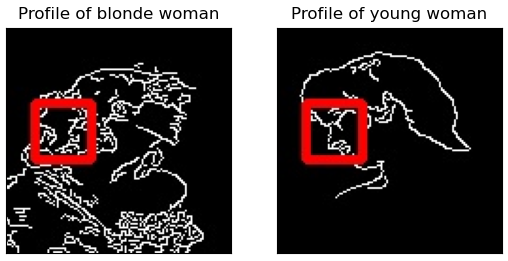
\includegraphics[width=0.90\textwidth]{./img/003.png}
            \caption{領域の位置の確認}
            \label{the position of a region}
        \end{figure}
    \end{center}
	この領域を縦方向にスキャンし、最初にエッジの画素にぶつかった位置をスタート地点に決める.
	\subsection{端点の検出と線の辿り方}
	\label{chap:end points detection}
	図4.1ではエッジが綺麗に繋がっているように見えるが、拡大すると途切れている. そのため、ロボットにそのままエッジの画素をそのまま座標として与えると実際の線画が点線になってしまう. そこで端点を用いる. 線の画素を辿り、端点まで来たら次に近くの端点へ移動して描いていく. この処理を行うことで実際には点線を描くことになるが、擬似的に線を描いていくような動作ができる.
	線の辿り方はある線の画素から隣に線の画素があるかを探し、線の画素があれば移動し、なければ最も近いまだ通過していない端点へと移動する. これを線の画素がなくなるまで繰りかえす.



  % -------------------------------------------------------------
  % 5章 実験
  %#! platex 000main.tex
\chapter{実験}
  \label{chap:experiment}
  \section{概要}
    \label{sec:summary}
	経路の求めるためにラスタスキャンと領域、端点を用いた方法のどちらが人のような描き方に近いかを比較し、どちらの描き順が人が描いたように見えるのかアンケートをoo人にとった.
  
  \section{比較手法}
    \label{sec:compare}
    比較には以下に示す
    \subsection{ラスタスキャン}
      \label{subsec:rastascan}

    \subsection{領域と端点を用いた方法}
      \label{subsec:mymethod}


  % -------------------------------------------------------------
  % 6章 結果
  %#! platex 000main.tex
\chapter{結果}
  \label{chap:result}
  表6.1はアンケート結果である. ほとんどの場合でラスタスキャンのほうが人に近いという結果がでた. 
  \begin{table}[h]
  \caption{アンケート結果\label{アンケート結果}}
  \label{tab:sample-tab}
  \begin{center}
      \vskip 1zh
      \small
      \begin{tabular}{c|c|c} \hline
        画像         & ラスタスキャン(人)   & 端点(人)  \\ \hline
       	1            & 6  				& 3   \\ 
        2            & 6	  			& 3   \\ 
        3            & 7   				& 2   \\ 
        4            & 6   				& 3   \\ 
        5            & 5   				& 4   \\ 
        6            & 5   				& 4   \\ 
        7            & 6   				& 3   \\ 
        8            & 2   				& 7   \\ 
        9            & 7   				& 2   \\ 
        10           & 6   				& 3   \\ \hline
      \end{tabular}
  \end{center}
\end{table}
  \section{考察}
  \label{sec:consideration}
  端点は線を辿るようにしたので,逆に一筆書きのようになり,不自然な書き方になったと考えられる. 実際に7枚の画像が目や鼻,耳などから頭上へ繋がって下から上へと描かれた.
  また,最も近い端点に移動すれば,近似的に線を描けると仮定したが,交点を考慮する必要があった. そのため,本来とは違う軌道になることが多くなったと考えられる. 
  エッジとノイズはトレードオフ関係にあるため,エッジを用いるなら,途切れた線を補間する必要があると考えられる.
  \section{描画の結果}
  \label{sec:drawing result}
  以下に今回用いたロボットに描画させた絵の画像を示す.


  
  %--------------------------------------------------------------
  % 7章 結論
  %#! platex 000main.tex
\chapter{結論}
  \label{chap:conclusion}
  本手法では, 端点を用いて人のような描き方ができるのかを調査した. 線を辿るように経路を生成したので,逆に一筆書きのようになった. 実際に多くの生成した経路が目や鼻,耳などから頭上へ繋がる下から上へ写る描かれ方をしていて,不自然な書き方になっていた.
  また最も近い端点に移動すれば, 近似的に線を描けると仮定したが, 途切れたエッジの補間や交点を考慮して経路を求めなかったため,望んだものとは少々違う軌道になることが多かった.
  全体としてラスタスキャンに方が優位であったが,生成結果は上から下へとプロッターのように単純な描き方であった.
  まとめると,線は上部から下部へと移り,それに加えて本手法のように線が繋がって描かれていると良いと考えられる.



  \backmatter
  %--------------------------------------------------------------
  % 謝辞
  %#! platex 000main.tex
%\chapter*{謝辞}
\chapter{謝辞}
  \label{chap:acknowledgments}


  %--------------------------------------------------------------
  % 参考文献
  %#! platex 000main.tex
\newlength{\oldbaselineskip}
\begin{thebibliography}{99}
	\bibitem{1}M. Pichkalev, R. Lavrenov, R. Safin and K. -H. Hsia, "Face Drawing by KUKA 6 Axis Robot Manipulator," 2019 12th International Conference on Developments in eSystems Engineering (DeSE), Kazan, Russia, 2019, pp. 709-714, doi: 10.1109/DeSE.2019.00132.
	\bibitem{2} Felix Fisgus, Joris Wegner:``Pankraz Piktograph''.
	\bibitem{3} Shubham Agarwal, Sarvesh S. S. Rawat, V Sumathi: ``A drawing robotic hand based on inverse kinematics'', International Conference on Information Communication and Embedded Systems (ICICES2014), Chennai, India, 2014, pp. 1-5, doi: 10.1109/ICICES.2014.7034005.
	\bibitem{4}D. Dhillon and R. Chouhan, "Enhanced Edge Detection Using SR-Guided Threshold Maneuvering and Window Mapping: Handling Broken Edges and Noisy Structures in Canny Edges," in IEEE Access, vol. 10, pp. 11191-11205, 2022, doi: 10.1109/ACCESS.2022.3145428.
	\bibitem{5}広瀬 茂男 著 機械工学選書 裳華房 ロボット工学-機械システムのベクトル解析-
	\bibitem{6}細田 耕著 実践ロボット制御-基礎から動力学まで-
	\bibitem{7}ディジタル画像処理(改訂第二版) 発行所 CG-ARTS (公益財団法人 画像情報教育振興協会)
\end{thebibliography}


  %--------------------------------------------------------------
  % 付録
  \newcounter{pageback}
  \setcounter{pageback}{\arabic{page}}
  \mainmatter
  \setcounter{page}{\arabic{pageback}}
  \addtocounter{page}{2}
  \appendix
  % 
  %#!platex 000main.tex

\end{document}
